\section{Basic concepts}
\label{sec:basic-concepts}

Before delving into the details of implementing the quantum circuit with error correction, a brief recapitulation about the basic concepts is helpful.
To keep it short, only the \emph{immediately needed} concepts are described.
It is assumed that the reader is already familiar with the principles of quantum computing.

\subsection{Quantum Error Correction}
\label{subsec:qec}

Error correction to fight noise has been around in the classical computing domain for a long time~\cite[p. 459]{benenti2004principles}.
It has been discovered that one of the key ingredients is \textbf{redundancy}~\cite[p. 459]{benenti2004principles}.
Fortunately the same happens to be true for the quantum domain~\cite[p. 46998]{Li}.
To apply a simple error correction one could use three instead of just one qubit carrying the same information just like in classical computing.
Unfortunately when dealing with qubits we have to obey some additional rules.

\begin{enumerate}
    \item There is the no-cloning theorem which means it is impossible to just copy quantum states~\cite[p. 460]{benenti2004principles}.
    We are left with encoding the same starting states of individual qubits or using \texttt{CNOT} gates to mimic copying behavior~\cite[p. 461]{benenti2004principles}.
    The approach using \texttt{CNOT} gates is shown in figure~\ref{fig:cnot-circuit}.
    \begin{figure}[H]
        \centering
        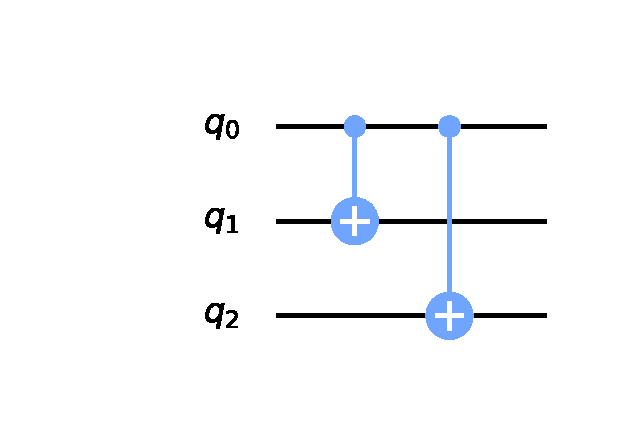
\includegraphics[width=0.5\textwidth]{res/cnot_circuit.pdf}
        \caption{\texttt{CNOT} gates used to encode the information of qubit \(q_0\) onto three.}
        \label{fig:cnot-circuit}
    \end{figure}
    \item Measuring a qubit causes its state to collapse~\cite[p. 460]{benenti2004principles}.
    Thus, we cannot just measure the state and correct it as it will destroy any superposition we ideally want to continue working with.
    The introduction of ancillary qubits that measure the \emph{error syndrome} solves that problem~\cite[p. 463]{benenti2004principles} as shown in figure~\ref{fig:reading-ancilla-qubits-circuit}.
    \begin{figure}[H]
        \centering
        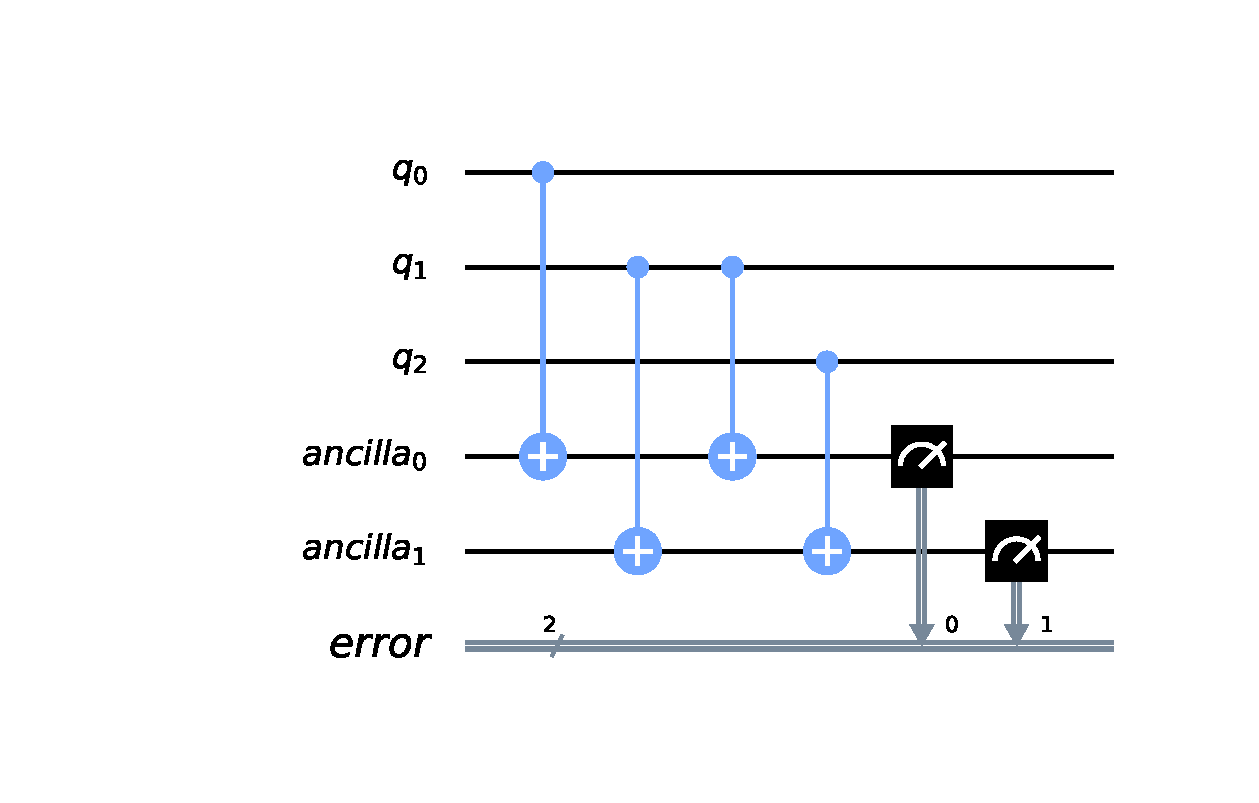
\includegraphics[width=\textwidth]{res/reading_ancilla_qubits_circuit.pdf}
        \caption{Measuring the \emph{error syndrome} using ancillary qubits.}
        \label{fig:reading-ancilla-qubits-circuit}
    \end{figure}
    The ancillary qubits under utilization of \texttt{CNOT} gates allow the comparison of the quantum information that is present in the redundant qubits.
    Thus, the following table shows the possible outcomes of the error syndrome which shows whether there was an error and even where it happened.
    \begin{center}
        \begin{tabular}{ r c l }
            \texttt{00} & \(\Rightarrow\) & No error happened \\
            \texttt{01} & \(\Rightarrow\) & Error happened in \(q_0\) \\
            \texttt{10} & \(\Rightarrow\) & Error happened in \(q_2\) \\
            \texttt{11} & \(\Rightarrow\) & Error happened in \(q_1\)
        \end{tabular}
    \end{center}
    Based on the results we are able to correct the errors.
    \item Compared to classical computing where only a bit-flip error is possible, qubits are additionally prone to phase-flips and even worse to a number of those errors.
    In the process of a quantum computation noise may apply multiple small rotations on the state~\cite[p. 460]{benenti2004principles}.
    \citeA[p. 465]{benenti2004principles} show that the same method for correcting bit-flips can be used to detect phase-flips when we transform from the \(\{|0\rangle, |1\rangle\}\) computational basis to \(\{|+\rangle, |-\rangle\}\) as a bit-flip becomes a phase-flip and vice versa.
\end{enumerate}

Since in this paper we will attempt to correct bit-flip errors, there is nothing more than this to understand how it works.

\subsection{Quantum Fourier Transform}
\label{subsec:quantum-fourier-transform}

In the course of this paper we try to correct errors in a quantum Fourier transformation (\emph{QFT}) algorithm.
Therefore, it is certainly advantageous to repeat the underlying concepts.

The QFT maps a quantum state \(|\psi\rangle\) on another quantum state \(|\alpha\rangle\) with the following definition~\cite[p. 1]{Weinstein_2001}.

\[
    QFT_M|\psi\rangle \rightarrow \frac{1}{\sqrt{M}} \sum_{k=0}^{M-1} e^{2 \pi i a k/M} |\alpha\rangle
\]

This can be expressed as a unitary matrix which can be decomposed into several quantum gates~\cite[p. 2]{Weinstein_2001}.
For example the one-qubit QFT is just the Hadamard gate~\cite{QiskitTBQFT}.

\[
    H = \frac{1}{\sqrt{2}}
    \begin{bmatrix}
        1 & 1 \\
        1 & -1
    \end{bmatrix}
\]

Another example is the two-qubit \(QFT_4\) taken from~\citeA[p. 2]{Weinstein_2001}.

\[
    QFT_4 = \frac{1}{2}
    \begin{bmatrix}
        1 & 1 & 1 & 1 \\
        1 & i & -1 & -i \\
        1 & -1 & 1 & -1 \\
        1 & -i & -1 & i
    \end{bmatrix}
\]

That matrix can be decomposed into the circuit shown in figure~\ref{fig:qft4-circuit}~\cite{QiskitTBQFT}.

\begin{figure}[H]
    \centering
    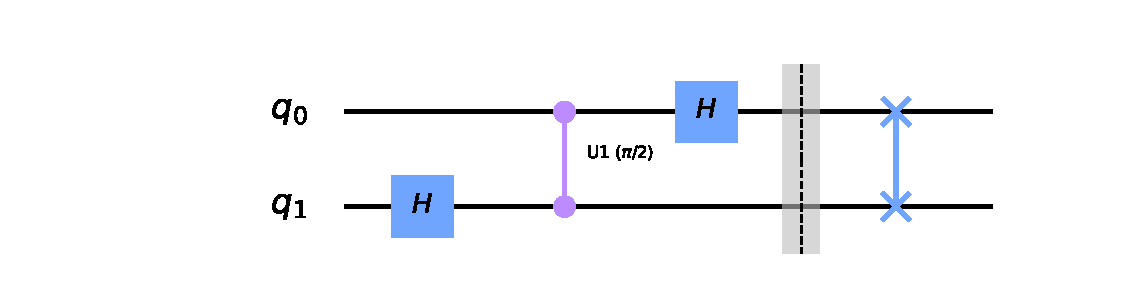
\includegraphics[width=0.7\textwidth]{res/qft4_circuit.pdf}
    \caption{Circuit for the two-qubit QFT \(QFT_4\).}
    \label{fig:qft4-circuit}
\end{figure}

\clearpage

All those matrices and circuits follow the same pattern~\cite{Yin2020Jun}:

\[
    QFT_M =
    \frac{1}{\sqrt{M}}
    \begin{bmatrix}
        1 & 1 & 1 & 1 & \ldots & 1 \\
        1 & \omega & \omega^2 & \omega^3 & \ldots & \omega^{M-1} \\
        1 & \omega^2 & \omega^4 & \omega^6 & \ldots & \omega^{2M-2} \\
        1 & \omega^3 & \omega^6 & \omega^9 & \ldots & \omega^{3M-3} \\
        \ldots & \ldots & \ldots & \ldots & \ldots & \ldots \\
        1 & \omega^{M-1} & \omega^{2M-2} & \omega^{3M-3} & \ldots & \omega^{(M-1)(M-1)} \\
    \end{bmatrix}
\]

where \(\omega = e^{\frac{2\pi i}{M}}\).
Even a matrix of any size can be broken down into a circuit as shown in Figure~\ref{fig:qft-generic-circuit}.
Note that the shown controlled \texttt{R} gate is really just a rotation around the Z-axis with angle \(\frac{\pi}{2^{k-1}}\).

\begin{figure}[H]
    \centering
    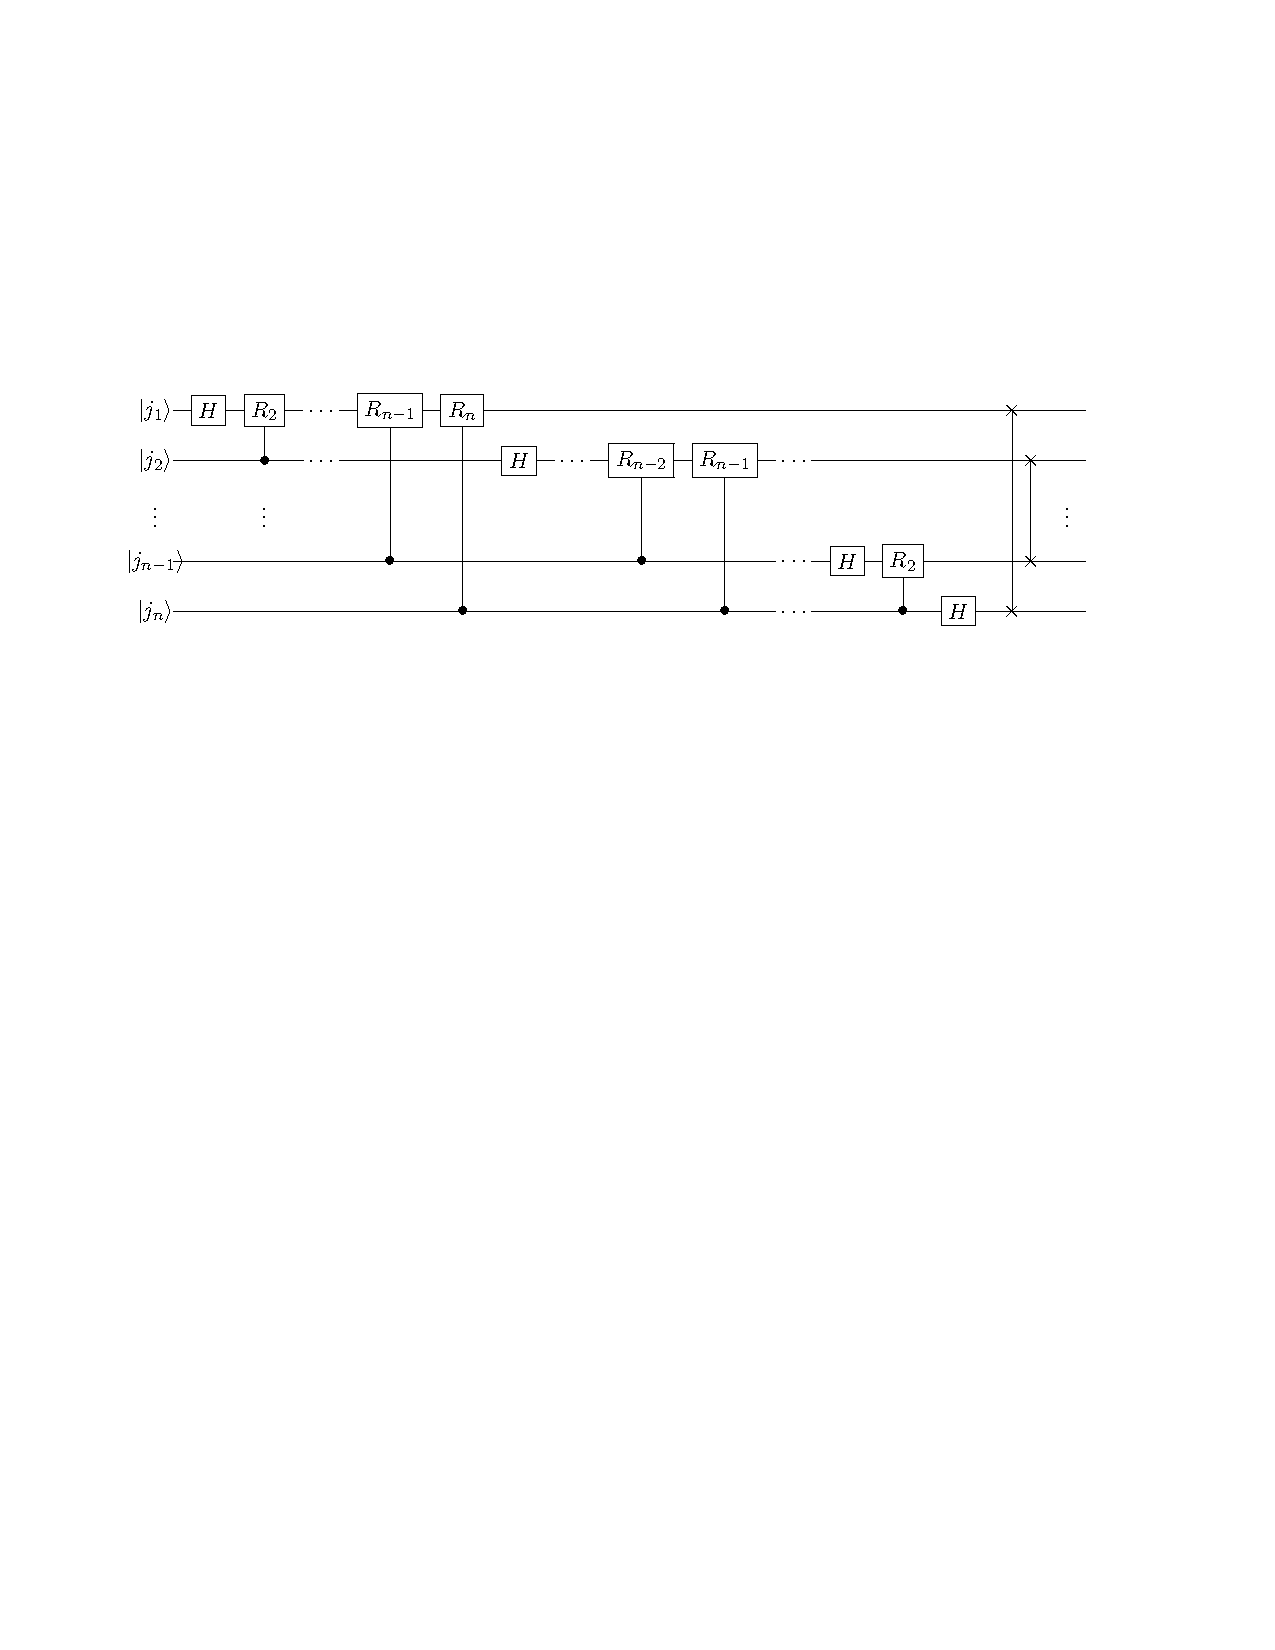
\includegraphics[width=\textwidth]{res/qftm_circuit.pdf}
    \caption{\(QFT_M\) circuit taken from \protect\citeA{VANJURGEN}}
    \label{fig:qft-generic-circuit}
\end{figure}

Now we have enough information at hand to realize such a circuit with the tools and methods introduced and used in the following sections.
